
\chapter{Beam elements}
\section{Classification of structures}
	\wrapfig{8}{l}{6.5}{0.45}{ch15/1}
	In the previous developpements we didn't need further information on the geometry, but they can help to simplify. In general we have the \textbf{3D solids}. When the thickness is much smaller than other dimensions, we have a: \\
	
	\begin{itemize}
	\item[•] \textbf{plate} if the structure is defined by a plane and if the main loading is transversal. 
	\item[•] \textbf{membrane} if the structure is loaded mainly within the plane
	\item[•] \textbf{shell} if the structure is curved or if the loads are in all directions.\\
	\end{itemize}
	
	If two of the dimensions are smaller than the third one, we speak of \textbf{straight beam} if the largest dimension follows a straight axis or \textbf{arch/curved beam} otherwise. If it carries only axial load, it is a \textbf{rod/bar} and if it is tension $\rightarrow$ \textbf{cable}, compression $\rightarrow$ \textbf{strut}.\\
	
	This classification is important because take for example a roof composed of beams supporting glass, modeling each beam in 3D would be inefficient since one or more directions are more relevant. Some simplifications can be made. 
	
\section{Beam theories}
	Beam in a plane, homogeneous isentropic linear elastic material. 
	
	\begin{center}
	\theor{
	\textbf{Euler-Bernouilli plane beam theory}\\
	
	\begin{itemize}
	\item[•] the vertical displacement (or deflection) of the points in a cross-section is small and equal to the deflection of the beam axis;
	\item[•] the lateral displacement (perpendicular to the plane) is equal to zero;
	\item[•] cross-sections normal to the beam axis remain plane and orthogonal to the beam axis after deformation (normal orthogonality condition).	
	\end{itemize}
	}
	\end{center}
	
	This theory is only valid for slender beams since the third condition means that there is no shear between axial fibers and this is only possible when the length is bigger than other dimensions ($\lambda = L/h > 100$). For thicker beams, \textbf{Timoshenko theory} is applied, the two first hypothesis holds true at the difference that the orthogonality is not preserved after deformation.
	
\section{2D Euler-Bernouilli finite elements}
	\wrapfig{7}{l}{6}{0.45}{ch15/2}
	For the further developments, we will assume that the material properties are constant over the material. Based on the figure the displacement field can be written as: 
	
	\begin{equation}
	\left\{ \begin{aligned}
	& u(x,y) = \bar{u}(x) - \phi (x)y\\
	& v(x,y) = v(x)
	\end{aligned}	
	 \right.
	\end{equation}
	
	where we separated the motion in axial and rotation ($\phi (x)= \frac{dv}{dx}$) at neutral axis. The fundamental variables and the \textbf{generalized strains} are derived as: 
	
	\begin{equation}
	q = \left[
	\begin{array}{c}
	\bar{u}(x)\\
	v
	\end{array}		
	\right]
	\qquad
	\epsilon = \left[
	\begin{array}{c}
	\bar{\epsilon}(x)\\
	1/R
	\end{array}		
	\right]
	= 
	\underbrace{
	\left[
	\begin{array}{cc}
	\frac{d}{dx} & 0 \\
	0 & \frac{d^2}{dx^2}
	\end{array}		
	\right]}_{D}
	\left[
	\begin{array}{c}
	\bar{u}(x)\\
	v
	\end{array}		
	\right]
	\end{equation}
	
		\wrapfig{6}{r}{7}{0.6}{ch15/3}
		where $\frac{1}{R} = \frac{d^2v}{dx^2}$ is the curvature of the beam. The generalized stress corresponding to the normal force and the bending moment can be defined as: 
	
	\begin{equation}
	\tau = \left[
	\begin{array}{c}
	N\\
	M
	\end{array}		
	\right]
	=
	\underbrace{
	\left[
	\begin{array}{cc}
	EA & 0\\
	0 & EI
	\end{array}		
	\right]}_{H}
	\epsilon
	\end{equation}
	
	where $A$ is the section area and $I$ the moment of inertia. The finite element method must account of the minimum order of continuity of the variables to approximate: \\
	
	\begin{itemize}
	\item[•] for $\vec{u}$, only the first order derivative is required, $C^0$ continuity is enough (value of $\vec{u}$ at nodes).  
	\item[•] for $v$, the second order derivative is needed, $C^1$ continuity is required (value of $v$ and $\frac{dv}{dx}$ at the node). \\
	\end{itemize}
	
	This gives 3 information per node, thus 6 DOF for the beam element. For the axial displacement, two values per element implies a linear shape function, while 4 values imply cubic function for $v$: 
	
	\begin{equation}
	u^e (x) = u_1 N_1 (x) + u_2 N_2 (x)\qquad v^e (x) = v_1 H_1 (x) + v_2 H_2 (x) + \phi _1 H_3(x) + \phi _2 H_4(x).
\end{equation}	 

	allowing to define the shape function matrix $N^e$ linking the displacements at x to the nodal values: 
	
	\begin{equation}
	u^e(x) = N^e (x)q^e = \left[
	\begin{array}{cccccc}
	N_1(x) & 0 &0 & N_2(x) & 0 & 0\\
	0 & H_1(x) &H_3(x) & 0 & H_2(x) & H_4(x)
	\end{array}
	\right] q^e.
	\end{equation}
	
	The shape function are constraints by the value they have to take at nodes 0 and $L$. 
	
	\begin{center}
	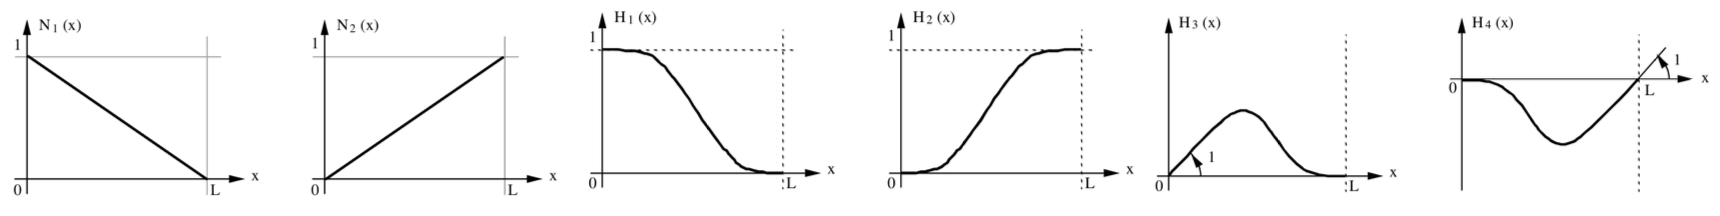
\includegraphics[scale=0.4]{ch15/4}
	\captionof{figure}{}
	\end{center}
	
	One can now compute the stiffness matrix by applying the integral and the nodal forces by assuming a uniform pressure $f^p = [p_x \ p_y]^T$ (see result p.113 it is too heavy). These expressions are based on a frame of reference on the beam, when we have to assemble a structure composed of several beams, we should use the common system called \textbf{structural axes}. This consists in multiplying by a rotation matrix: 
	
	\begin{equation}
	q^e = [u_1^e \ v_1^e \ C_1^e \ u_2^e \ v_2^e \ C_2^e] = \left[ 
	\begin{array}{cccccc}
	\cos (\theta) & \sin (\theta) & 0 & 0 &0&0\\
	-\sin (\theta) & \cos (\theta) & 0 & 0 &0&0\\
	0 & 0 & 1 & 0 & 0 & 0\\	
	0 & 0 & 0 & \cos (\theta) & \sin (\theta) & 0\\	
	0 & 0 & 0 & -\sin (\theta) & \cos (\theta) & 0\\	
	0 & 0 & 0 & 0 & 0 & 1\\		
	\end{array}
	\right]
	 [u_1^{e,s} \ v_1^{e,s} \ C_1^{e,s} \ u_2^{e,s} \ v_2^{e,s} \ C_2^{e,s}] 
	\end{equation}
	
	where $q^e$ are the displacements in local axis, $q^{e,s}$ in structural axis and $\theta$ the angle of rotation. Same applied to the forces, we can rewrite the stiffness relation as:
	
	\begin{equation}
	K^e q^e = f^e \Rightarrow K^e R^e q^{e,s} = R^e f^{e,s}\Rightarrow R^{e^{-1}} K^e R^e q^{e,s} = R^{e^{-1}}R^e f^{e,s}\qquad \Rightarrow K^{e,s} q^{e,s} = f^{e,s}
	\end{equation}
	
	It can be proven that this approach gives exact values at the nodes for constant $EI$.